% !TEX root = ../master.tex
\chapter{Design and Methodology}
\label{chap:design}
TODO forcast



\section{Employed Methodology}
TODO


general method:
design science research / constructive research
\url{https://en.wikipedia.org/wiki/Constructive_research}
\autocite[][]{dresh2015designresearch}
but with focus on "practical utility"
therefore:
1. fuzzy sources: manual literature review that lead to fundamentals
2. theoretical body of knowlede: cullected in fundamentals
3. relevant problem: 
    - volume detectoin might hold the opportunity to further improve efficiency with the degree of usage on elevators
    - limited by 80\% oder auch 60-70\% rule \autocite[][p.~194]{unger2015aufzuege} ??, unused capacity (referece)
    - also detection of bigger items such as janitors cars, baby buggies  might be useful
4. solution construction: using engineering methods
    also:    
    - set objectives and tasks: see research questions
    - identify process model
    - select case execution
    - interview case organization
    - prepare simulation / test
    - run simulation / test
    - interpret simulation /test results
    - give feedback
5. practical relevance: interpretation of test results and considerations of marketing and economic value and need of the solution

theoretical relevance and contribution to theoretical body are not conducted

\begin{figure}[hbt]
	\centering
	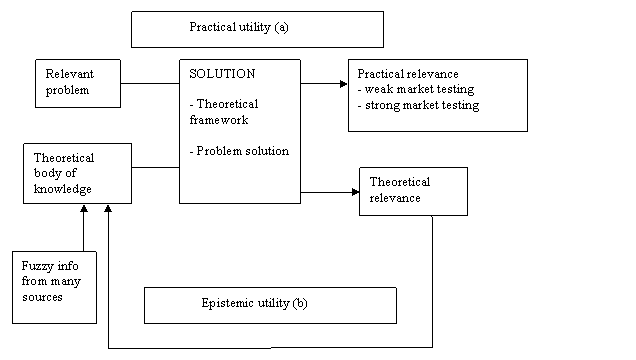
\includegraphics[width=0.8\textwidth, keepaspectratio]{resources/Rasvan_constructive_research_diagram.gif}
	\caption{\label{fig:design:constructiveresearch} Components of constructive research. Source }
\end{figure}


come back to research questions an look onto what strategy is used to answer them

twofold:
1. design and implementation of system to gather volume data of passengers
 - find current system architecture
 - define positions to integrate new components
 - define what information should come out of the system
 (eg passenger numbers, position, tracking, volume, other objects)
 - find and choose standard algorithms for passenger detection and volume estimation in visual system (taken from fundamentals)
 - match algorithm and hardware setup possibilities
 - implement detection system
 - test detection system exemplary by filming an elevator cabin and the outside (detection system not yet influencing the elevator system)
 
2. integration of volume passenger data into existing scheduling algorithm
 - define suitable elevator configuration that can benefit from solution (taken from fundamentals) 
 - find standard algorithm for this configuration (taken from fundamentals)
 - find an integration point for the data gathered by 1.
 - compare the two algorithms effectiveness by running a simulation with the same parameters for both to check if it is even relevant to use this advanced information
 
 TODO: mapping between upper, theoretical description of method and  lower actual conduction.
 
 
 TODO rework the nexts sections according to the method defined above, also: which is design, which is implementation?

\section{Requirements}
TODO

\autocite[][]{xang2016trafficlist} has done tehe same and patentet it :(

\section{Conduction of Method}
TODO the method determines which steps to take
TODO, choose possible approach from sota

\section{Proposed Solution}
TODO next two are included?

\section{Architectural Plan}
TODO necessary? yes

\section{Algorithmic Approach}
TODO necessary? yes

\section{Validation Strategy}

TODO